\documentclass{article}
\usepackage[utf8]{inputenc}
\usepackage[top=2cm, bottom=2cm, left=1.5cm, right=1.5cm]{geometry}
\usepackage{amsmath,amsfonts,amssymb, mathtools}
\usepackage{color}
\usepackage{caption}
\usepackage{hyperref}
\captionsetup{figurename=Fig,font=scriptsize}
\usepackage{subcaption}
\usepackage{enumitem}
\newtheorem{Def}{Définition}

\title{Dataiku exercice : US Census Data Set}
\author{Bénédicte RALLET}
\date{Programming Langage : R}

\begin{document}
\maketitle
\vspace{2cm}
\tableofcontents
\newpage
\section{Statistic based and univariate audit}
\noindent The data set from the US Census contains 42 variables but one of them is not used ("instance weight") and one corresponds to the variable that we want to predict. Thus, we have a total of 40 available predictors to fit a model. 7 are continuous variables and 33 are nominal ones.
\subsection{General information}
\vspace{0.5cm}
\begin{center}
\begin{tabular}{|c|c|c|c|c|}
\hline
 \textbf{Variable} & \textbf{Code} & \textbf{Type} & \textbf{Missing values "?"} & \textbf{NIU}\\
 \hline
 age & AAGE & Continuous & &\\
 \hline
 class of worker & ACLSWKR & Nominal (9 levels) & & 100245\\
 \hline
 industry code & ADTIND & Nominal (52 levels) & & \\
 \hline
 occupation code & ADTOCC & Nominal (47 levels) & &\\
 \hline
 education & AHGA & Nominal (17 levels) & &\\
 \hline
 wage per hour & AHRSPAY & Continuous & &\\
 \hline
 enrolled in edu inst last wk & AHSCOL & Nominal (yes/no/NIU) & & 186943\\
 \hline
 marital status	& AMARITL & Nominal (7 levels) & &\\
 \hline
 major industry code & AMJIND & Nominal (24 levels) & & 100684\\
 \hline
 major occupation code	& AMJOCC & Nominal (15 levels) & & 100684 \\
 \hline
 race	& ARACE & Nominal (5 levels) & &\\
 \hline
 hispanic origin & AREORGN & Nominal (10 levels) & &\\
 \hline
 sex & ASEX & Binary & &\\
\hline
 member of a labor union & AUNMEM & Nominal (yes/no/NIU) & & 180459\\
\hline
 reason for unemployment & AUNTYPE & Nominal (6 levels) & & 193453\\
\hline
 full or part time employment stat & AWKSTAT & Nominal (8 levels) & &\\
\hline
 capital gains & CAPGAIN& Continuous & &\\
\hline
 capital losses & CAPLOSS & Continuous & &\\
\hline 
 divdends from stocks & DIVVAL & Continuous & & \\
\hline
 tax filer status & FILESTAT & Nominal (6 levels) & &\\
\hline
 region of previous residence & GRINREG & Nominal (6 levels) & & 183750\\
\hline
 state of previous residence & GRINST & Nominal (51 levels) & 708 & 183750\\
\hline
 detailed household and family stat & HHDFMX & Nominal (38 levels) & &\\
\hline
 detailed household summary in household & HHDREL & Nominal (8 levels) & &\\
\hline
 migration code-change in msa & MIGMTR1 & Nominal (10 levels) & 99696 & 1516\\
\hline
 migration code-change in reg & MIGMTR3 & Nominal (9 levels) & 99696 & 1516\\
\hline
 migration code-move within reg & MIGMTR4 & Nominal (10 levels) & 99696 & 1516\\
\hline
 live in this house 1 year ago & MIGSAME & Nominal (yes/no/NIU) & & 101212\\
\hline
 migration prev res in sunbelt & MIGSUN & Nominal (4 levels) & 99696 & 84054\\
\hline
 num persons worked for employer & NOEMP & Continuous & &\\
\hline
 family members under 18 & PARENT & Nominal (5 levels) & & 144232\\
\hline
 country of birth father & PEFNTVTY & Nominal (43 levels) & 6713 &\\
\hline
 country of birth mother & PEMNTVTY & Nominal (43 levels) & 6119 &\\
\hline
 country of birth self & PENATVTY & Nominal (43 levels) & 3393 &\\
\hline
 citizenship & PRCITSHP & Nominal (5 levels) & & \\
\hline
 own business or self employed & SEOTR & Nominal (3 levels) & &\\
\hline
fill veteran's admin & VETQVA & Nominal (3 levels) & & 197539\\
\hline
veterans benefits &	VETYN & Nominal (3 levels) & &\\
\hline
weeks worked in year & WKSWORK & Continuous & & \\
\hline
year & YEAR & Nominal (94 or 95) & & \\
\hline
\end{tabular}
\end{center}
\vspace{0.3cm}
\noindent \underline{Note} : "NIU" stands for "Not In Universe"
\newpage
\subsection{Continuous variables}
\textbf{Age}\\

\noindent The variable \textit{AAGE} is a continuous variable witch takes its values from $0$ to $90$. We can represent the variable using a boxplot to see the general distribution of the variable. We can see that the median is around 30 years and half of the population has an age between 15 and 50 years old.\\In addition, we can plot an histogram, where the interval is 10 years. We can notice that the most represented category is the one between 0 and 10 years. This is an information that we didn't see with the boxplot.\\
\begin{center}
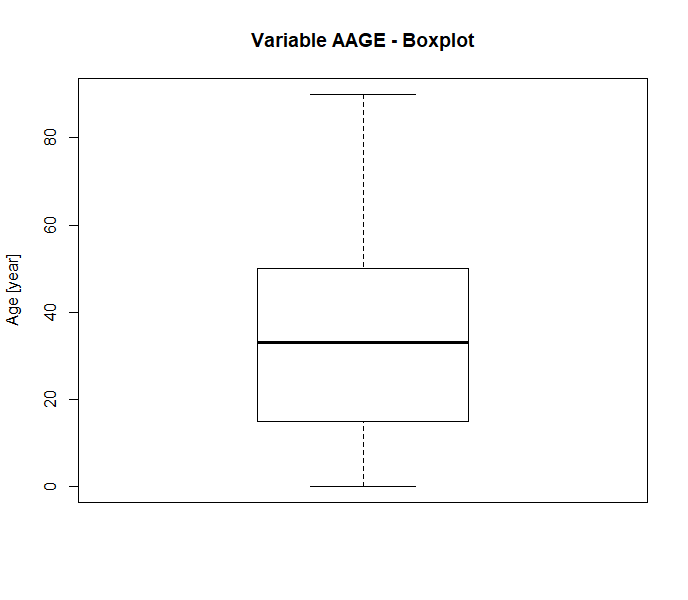
\includegraphics[width = 8cm]{AAGE_boxplot.png}
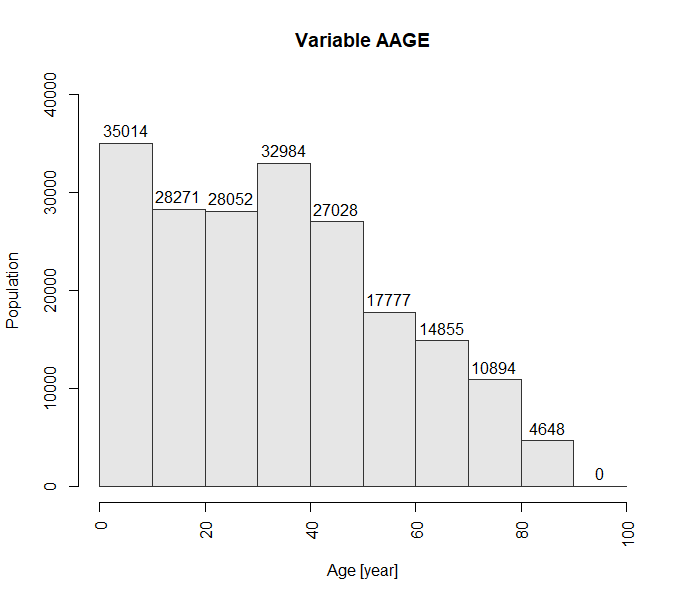
\includegraphics[width = 8cm]{AAGE_hist.png}
\end{center}

\noindent\textbf{Wage per hour}\\

\noindent With R, we can obtain a statistical summary of the variable \textit{AHRSPAY}. The result shows that more than 75\% of the values are 0. There is indeed 94.44\% of values equal to 0 in the data set. Plotting a boxplot with all the values will not show anything.\\
\begin{center}
\begin{tabular}{c|c|c|c|c|c}
Min. & 1st Qu. &  Median & Mean & 3rd Qu. & Max. \\
\hline
0.00 & 0.00 & 0.00 & 55.43 & 0.00 & 9999.00 \\
\end{tabular}
\end{center}

\noindent A solution could be to plot only the non-zero value to have an idea of the distribution of the 5.66\% values different from 0. The visual result is still not really good because there is a lot of extreme values.\\
\begin{center}
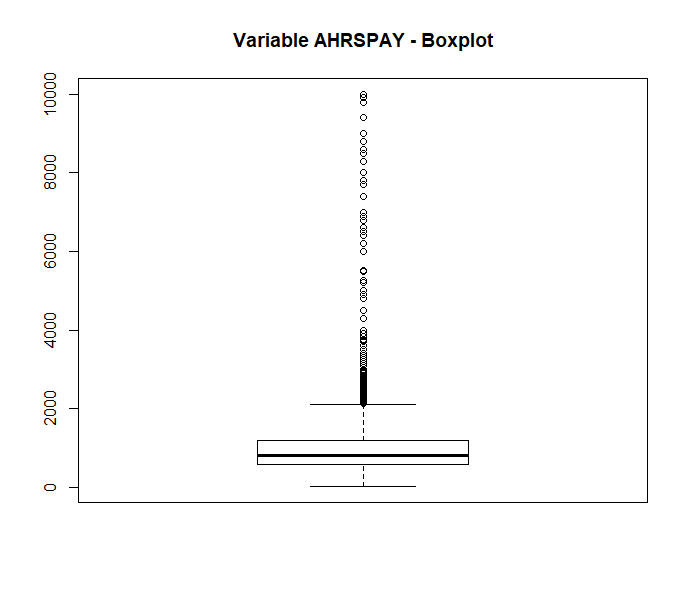
\includegraphics[width = 8cm]{AHRSPAY.png}
\end{center}

\noindent\textbf{Capital gains, losses and dividends from stocks}\\

\noindent As previously, these variables have a majority of zero-values which make difficult to have a graphical representation of the distribution of the variable. The percentages of non-zero values are the following :
\begin{itemize}
    \item \textit{CAPGAIN} : 3.70\%
    \item \textit{CAPLOSS} : 1.96\%
    \item \textit{DIVVAL} : 10.96\% 
\end{itemize}

\vspace{0.5 cm}
\noindent\textbf{Persons work for employer}\\

\noindent The summary of the variable \textit{NOEMP} shows that the variable takes its value between $0$ and $6$, with a mean of almost 2 persons employed.\\
\begin{center}
\begin{tabular}{c|c|c|c|c|c}
Min. & 1st Qu. &  Median & Mean & 3rd Qu. & Max. \\
\hline
0.000 & 0.000 & 1.000 & 1.956 & 4.000 & 6.000  \\
\end{tabular}
\end{center}
\begin{center}
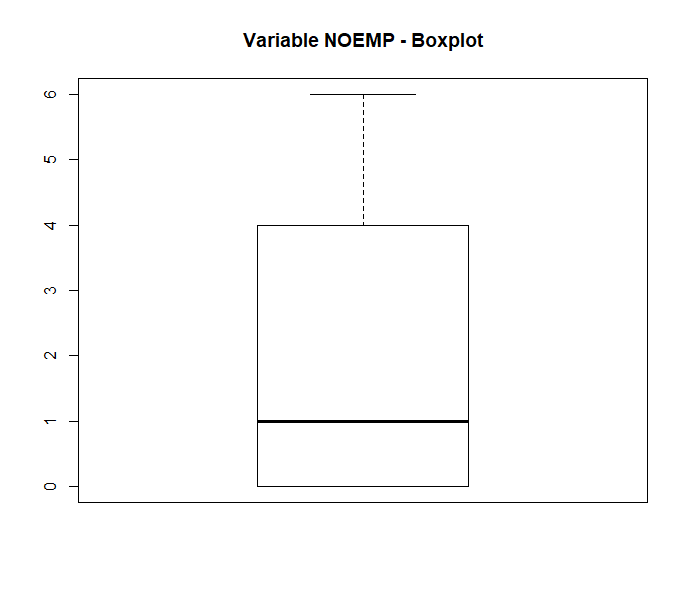
\includegraphics[width = 6cm]{NOEMP.png}
\end{center}

\noindent\textbf{Weeks worked in year}\\

\noindent With the histogram below, we clearly see that most of the people are either working 0 week (not working tough) or 52 per year. 96.3\% of the population of the data set is in one of these cases.\\
\begin{center}
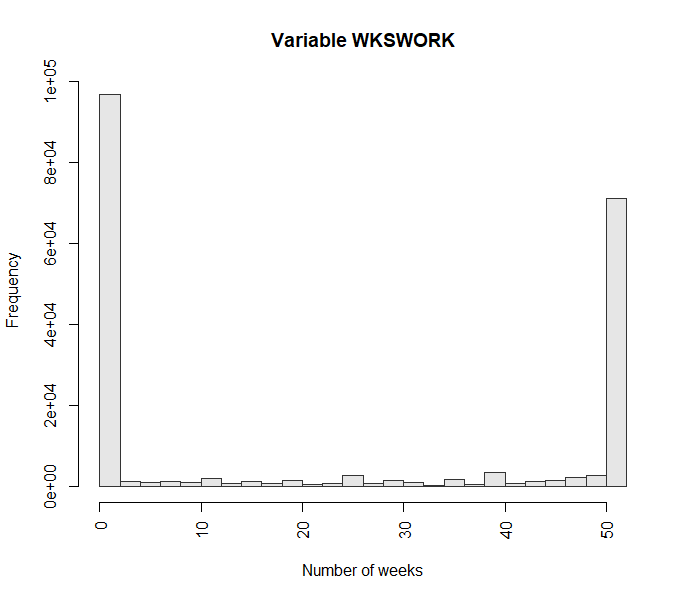
\includegraphics[width = 9cm]{WKSWORK.png}
\end{center}

\newpage

\subsection{Nominal variables}
\noindent The other variables are quantitative variables, interpreted as "factor" by R. \\
There are different ways to show the distribution of this type of variables : barplot, pie chart, histogram...
Nevertheless, it can be tricky sometimes to have a nice visual chart when there are too many categories. The chart become messy and it is hard to distinguish
the different values.\\

\noindent The following charts are representations for the variables \textit{ASEX}, \textit{ARACE}, \textit{AMARITL}, \textit{AMJIND}, \textit{GRINREG} and \textit{AHGA} (that shows how it is
difficult to visualise a chart with a high number of categories).\\

\noindent This list is not exhaustive and other descriptive charts can be found at \url{https://github.com/benrallet/Dataiku_US_Census/tree/master/Charts}. \\

\begin{center}
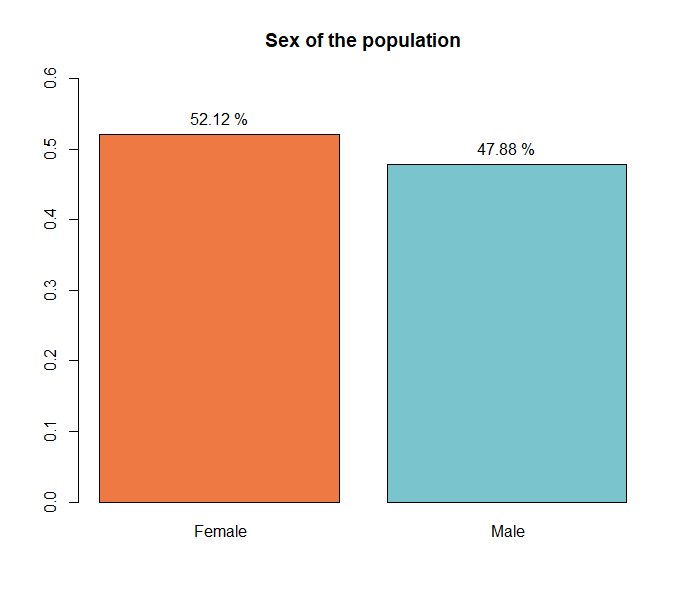
\includegraphics[width=8.5cm]{ASEX.png}
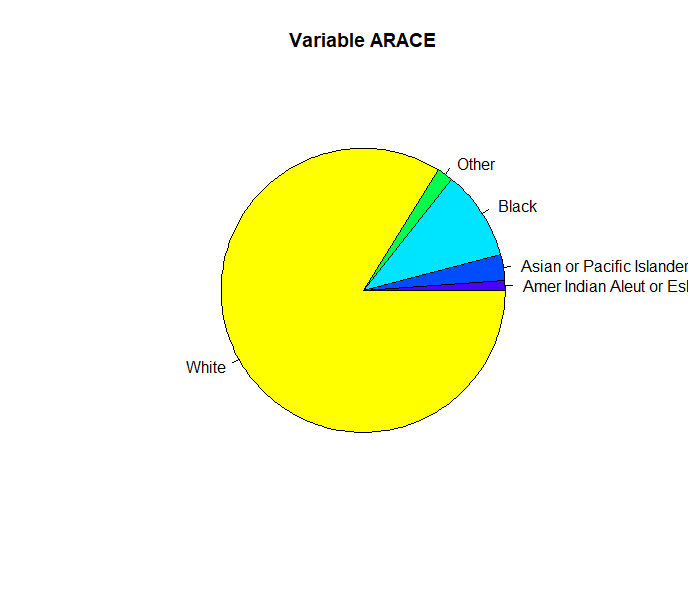
\includegraphics[width=8.5cm]{ARACE.png}\\
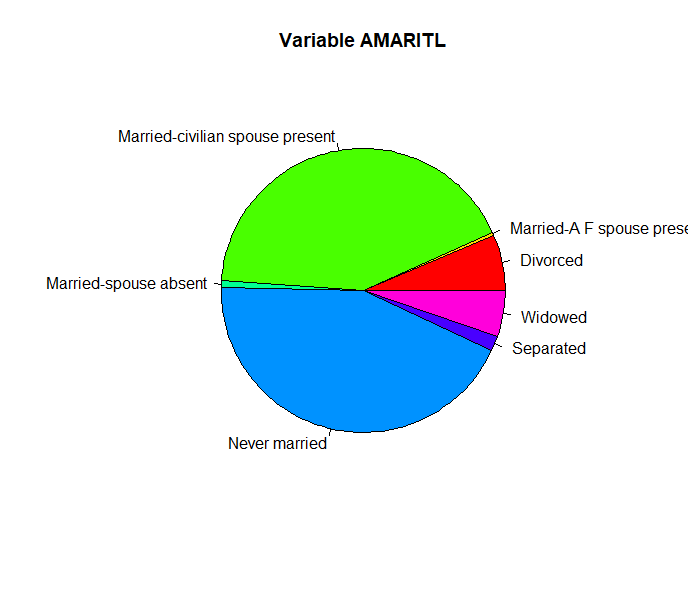
\includegraphics[width=8cm]{AMARITL.png}
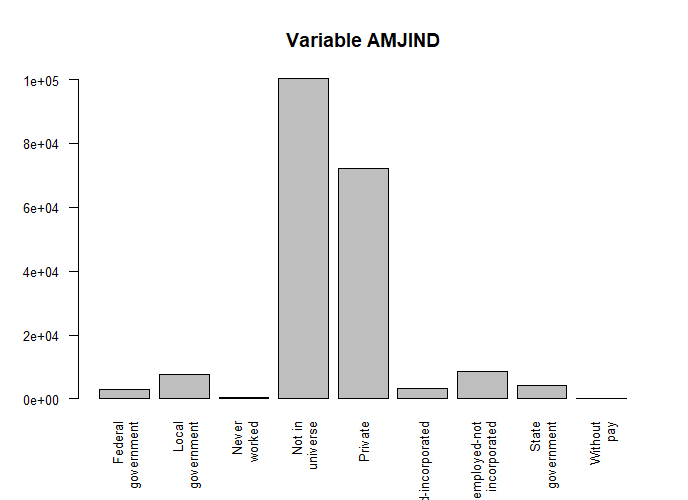
\includegraphics[width=10cm]{AMJIND.png}\\
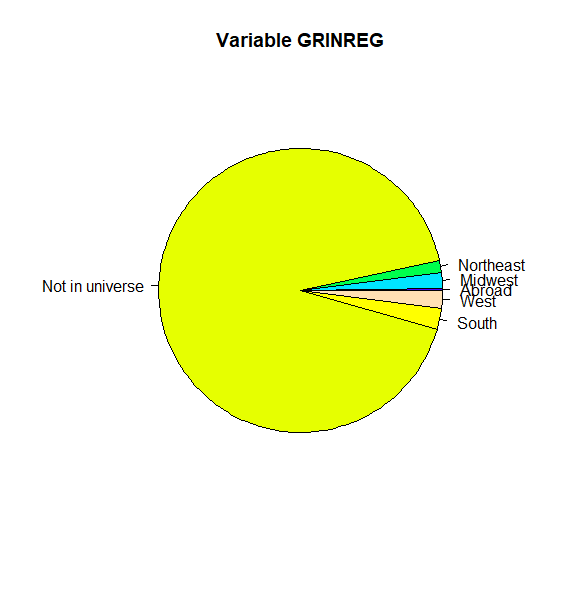
\includegraphics[width=8cm]{GRINREG.png}
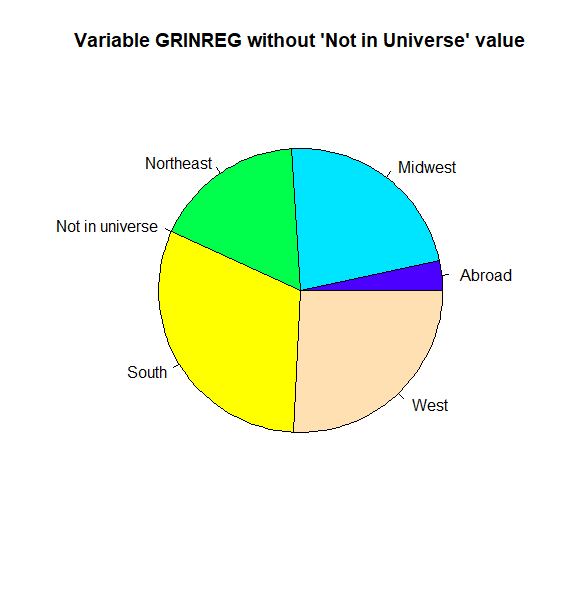
\includegraphics[width=8cm]{GRINREG2.png}\\
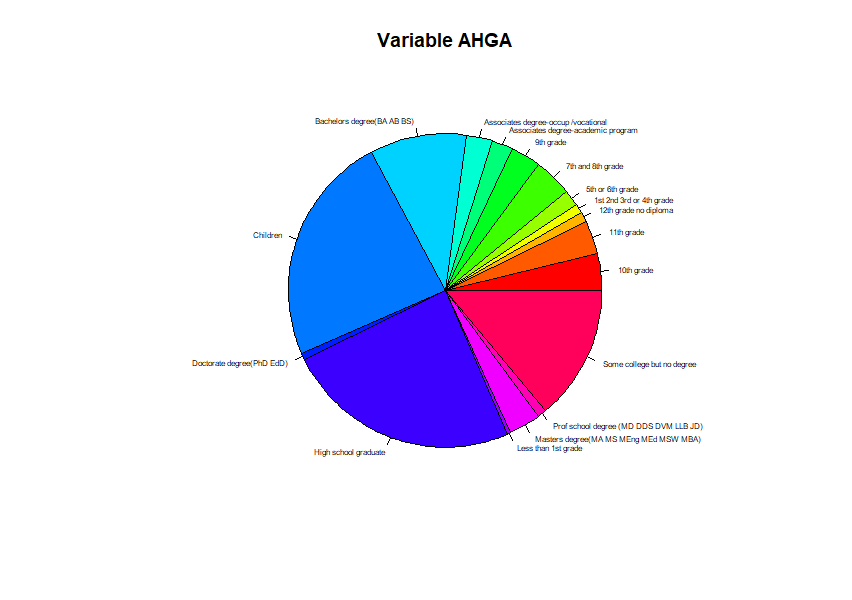
\includegraphics[width=18cm]{AHGA.png}
\end{center}
\newpage
\section{Creation of a model}
\noindent In this part, we will test two algorithms on our training set : decision tree and logistic regression.\\ After pre-processing the data, the algorithms will be implemented and their performance (error rate) will be computed using 10-Fold Cross-Validation. According to these results, one model will be chosen to model wining more or less than \$50,000/year for the test data. 
\subsection{Decision Tree}
Presentation of the steps followed to create a decision tree : \\

\noindent\textbf{Pre-processing data} \\

\noindent To model the decision tree, I will be using the library \textit{tree} available as a package with R. \\

\noindent From an implementation point of view, one big advantage of the decision trees is that they can deal with both categorical and continuous variables. However, one limit with the library used is that it can't handle categorical variables with more than 32 levels.\\

\noindent In our case, seven variables don't fill this condition.
\begin{itemize}
    \item Industry and Occupation code : these two variables have, respectively, 52 and 47 different values. However, a "major" category exists for each of these variables (Major industry code and Major occupation code) that regroup some categories to have a lower number of levels. For the aim of this exercise, I admit that the major variables will be enough to represent an observation.
    \item State of previous residence : this variable has 51 different values. A variable representing the region of previous residence is also in the data set. Regions can be seen as an aggregation of states. Thus, I made the choice to simply remove this variable to fit the model. 
    \item Detailed Household and Family Stat : as the previous variables, it exists a predictor called "detailed household summary" that has only 8 levels (against 38 for the other one). I chose to remove also this variable from our model.
    \item Country of birth of the father, the mother and self (three variables) : these three variable have each one 43 categories corresponding to countries. To reduce this number, I thought about different solutions : grouping by continent, one-hot encoding, USA/not USA. I finally chose the last option as it does not increase the number of predictor and it was quite easy to set up. The three variables will now be used as binary predictors, 1 corresponding to United-States and 0 to others.
\end{itemize}

\noindent In this four cases, there is a loss of information but the information does not completely disappear (trade-off). \\

\noindent\textbf{Construction of the tree} \\

\noindent To create the decision tree with the $tree$ library, 
\begin{enumerate}
    \item function \textit{tree} to fit the model. The parameter \textit{tree.control(nobs=dim(trainData)[1],mindev = 0.0001}) is used to have a complete tree.
    \item \textit{cv.tree} construct the sequence of the sub-trees embedded in the one obtained with function \textit{tree} and to estimate the error rate with cross-validation
    \item prune.misclass is used to do pruning based on the error rate estimation from the previous step
    \item finally, \textit{predict} gives the responses for a data set based on the decision tree constructed 
\end{enumerate}

\vspace{0.5cm}
\noindent\textbf{Computation of the error rate} \\

\noindent Once we have the responses for a data set (all variables but the output variables), we have to compare them to the "real" response, contained in the last column of the data set. Let $pred$ be the array of predictions from the model and $z$ the array of reality predicitions. The error rate can be computed as follow : \\

$$error = \frac{1}{n}\sum_{i=1}^{n}I(pred_i \neq z_i)$$
\noindent where n is the number of observations and I is a function that returns 1 if $pred_i \neq z_i$ and 0 otherwise.\\

\subsection{Logistic Regression}
\noindent\textbf{Pre-processing data} \\

\noindent For the logistic regression model, more pre-processing had to be done. Indeed, the algorithm can't handle categorical variables. Most of the predictors being categorical variables, a solution had to be implemented.\\

\noindent First, I applied the same transformation and removed the same variables than for the decision tree model. I simplified the model and removed the variable with a lot of factors than could lead to a big number of dummy variables (see the section corresponding).\\

\noindent Then, I transformed the variables $ASEX$ and $YEAR$ into binary variable (0/1). The transformation was immediate because they had only two categories. \\
\noindent To transform the other categorical variables (with more than two levels) to a binary variable, I used one-hot encoding. Integer encoding couldn't work because there were no ordinal relationships between the categories. \\

\noindent\textbf{Fit the logistic regression model} \\

\noindent First, I used the \textit{glm()} function of R, with \textit{family="binomial"} to fit a logistic regression model. The one-hot encoding strategy increased a lot the number of variables of our model and, because of the curse of dimensionality, the algorithm didn't converge. \\

\noindent To fix this issue, I used a shrinkage method, called \textbf{lasso} to perform both variable selection and regularization. The aim of this method is to improve the prediction accuracy as well as the interpretability of the model. Contrary to the ridge regression method, it does not necessary keep all the predictors in the final model. Thus, we can easily see which predictors don't have much importance in the prediction and, on the other side, the ones which play the biggest roles to predict the output.\\

\noindent This method is available with the R library \textit{glmnet}. I used the function called \textit{cv.glmnet}. I set $\alpha$, the elasticnet parameter, to 1 (the lasso penalty) and \textit{nfolds}, the cross-validation parameter to find the optimal $\lambda$, to 5.\\
Once the cross-validation for \textit{glmnet} is done, we can predict the income level by using a specified $\lambda$. I chose to use the $\lambda$ that minimizes the mean cross-validated error. \\

\noindent With this method, we can get the coefficients for each variable with \textit{coef()}. The variables that are assigned to 0 are not used to construct the model. For the others, if the variables are standardized before fitting the model, we can compare the variable coefficients to evaluate their importance.

\newpage
\subsection{Performance comparison and choice of the model}
\noindent To estimate the error rate of the two models, I used \textbf{cross-validation}.\\ 

\noindent In my case, I chose to implement a 10-Fold Cross-Validation. It means that we separate randomly our training data set into 10 different groups of approximately the same size. We use the first fold as a validation set and the nine others to fit the model. We compute an error rate that we will call $MSE_i$. We repeat this procedure $k-1$ using the $k-1$ other folds, one after one, as the validation set and we fit a new model. \\

\noindent At the end, we compute the CV Error Rate :
$$CV = \frac{1}{k}\sum_{i=1}{k}MSE_i$$

\noindent The results obtained with the two algorithms are the following :\\

\begin{tabular}{c|c|c}
    Model & CV Error Rate & 95\% CI  \\
    \hline
    Logistic regression  & $0.04798946$ & $[0.04730451, 0.04867440]$ \\
    Decision Tree & $0.04864101 $ & $[0.04777509, 0.04950693]$\\
\end{tabular}

\vspace{0.5cm}
\noindent According to these results, there isn't a significant difference between the two models. Indeed, the 95\% confidence interval are overlapped. \\

\noindent Thus, I chose to keep the decision tree model for different reasons. First, there is less pre-processing to do with the data set. Then, as there is no one-hot encoding data, it is easier to interpret the results. The variables have kept their original names.
\newpage
\section{Application of the model on the test file}

We will now train our decision tree model with all the training set. \\
We have to apply the same modification to the test data that we did to the training data to fit the model.\\

\noindent\textbf{Error rate} \\

\noindent We obtain a test error rate of \textbf{4.81\%} with our decision tree model.\\

\noindent Less than 5\% of error rate is a good result in absolute terms. Nevertheless, we have to be careful with this number. Indeed, there is a very low number of observations with the label "+50000". For the training set, 6.2058\% of the population has this label and 6.2008\% for the test set. It means that a classifier that would always predict the response "-50000" would have an error rate of around 6.20\%.\\

\noindent\textbf{Confusion Matrix} \\

\noindent To see where the classifier made mistakes in its prediction, we can show the confusion matrix.\\

\begin{tabular}{cc|c|c}
\multicolumn{2}{c|}{}& \multicolumn{2}{c}{Predicted} \\
\multicolumn{2}{c|}{} & Positive &	Negative\\
\hline
Observed &	Positive &	92289 & 1287\\
\cline{2-4} 
& Negative & 3517 & 2669
\end{tabular}

\vspace{0.5cm}
\noindent We can also compute other indicators as the sensitivity, equal to 0.9633, and the specificity, equal to 0.6747.  \\

\noindent\textbf{Importance of predictors} \\

\noindent With our library, we can get the variables that were used in the decision tree :\\

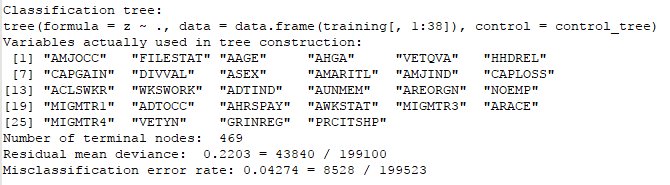
\includegraphics[width = 12cm]{tree_summary.png}

\vspace{0.7cm}

\noindent Using this result, we can do more in-depth analysis of some of these variables, especially the ones used at the top of the decision tree. It can help us to draw a profile of the people that make more than \$50,000 per year.\\

\newpage
\begin{enumerate}
    \item Major Occupation Code\\
    
This variable represents the field in which the person is working. The following table is a table that shows, for each level, the proportion of person in each category of the \textit{AMJOCC} variable. I chose to show the proportion because the two levels of income don't have the same number of observations. In this way it is easier to compare both repartition.
\begin{center}
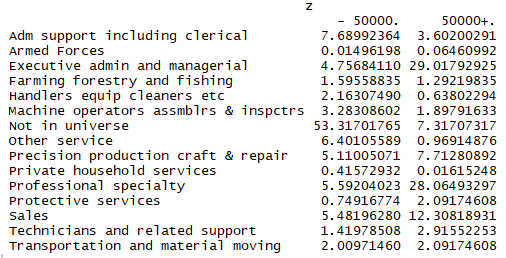
\includegraphics[width=10cm]{AMJOCC_table.png}
\end{center}
We can see that almost 70\% of the "50000+" people are in three categories: Executive admin and managerial, Professional specialty and Sales. 

    \item Tax Filer Status\\

We present the same type of table for this variable.
\begin{center}
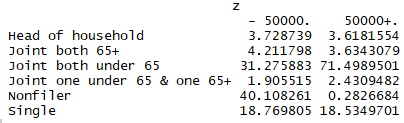
\includegraphics[width=8cm]{FILESTAT_table.png}
\end{center}
90\% of people that make more than \$50000 per year are either "Joint both under 65" or "Single". However, there is the same proportion of single people in both categories of income level whereas the proportion of "Joint both under 65" is more than the double in the case of "+50000". On the other side, we see that it is really rare for a "Nonfiler" to earn more than \$50000 a year.

    \item Age\\
    
The variable \textit{AAGE} is continuous so we can plot a boxplot for each income level.
\begin{center}
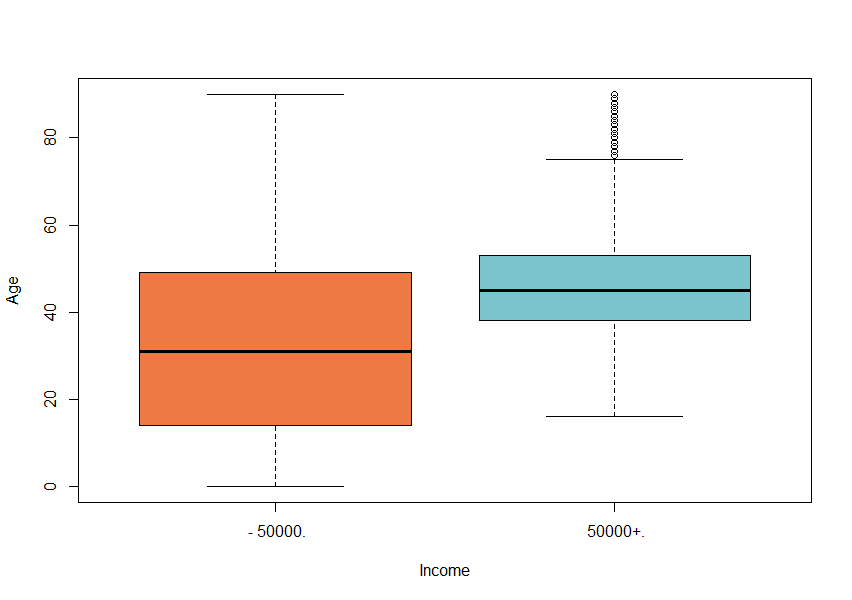
\includegraphics[width=8cm]{AAGEz.png}
\end{center}
We can clearly see that the mean of "50000+" people is higher than the mean of the others. The age of 75\% of the observations for this category is between 38 and 53 years old.  

    \item Education \\
\begin{center}
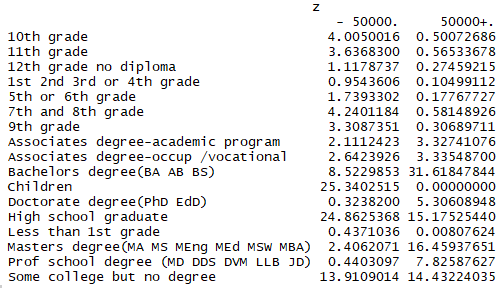
\includegraphics[width=9cm]{AHGA_table.png}
\end{center}
The education level the most represented for the person that earn more than \$50000/year is "Bachelor degrees" (around 30\%), followed by "High School Graduate", "Master Degree" and "Some college but no degree".

    \item Weeks worked per year \\
\begin{center}
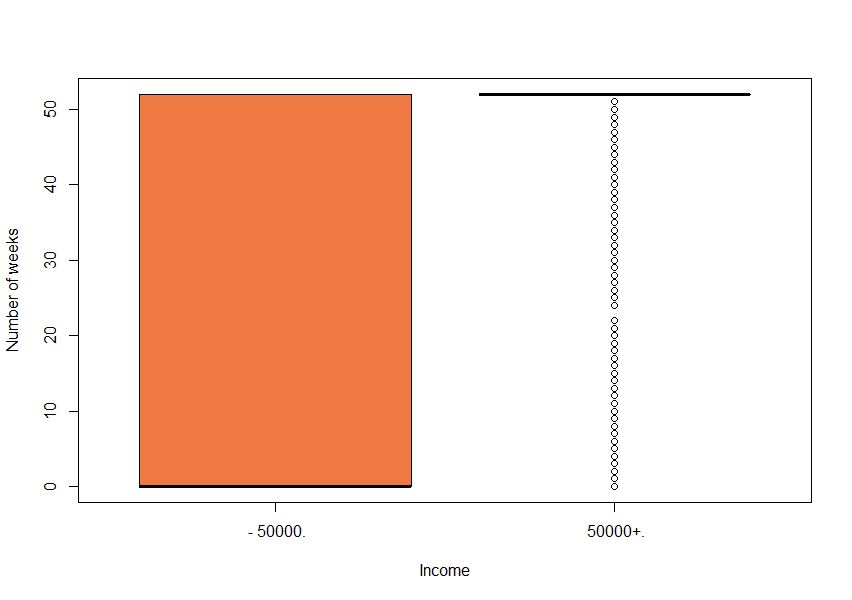
\includegraphics[width=9cm]{WKSWORKz.png}
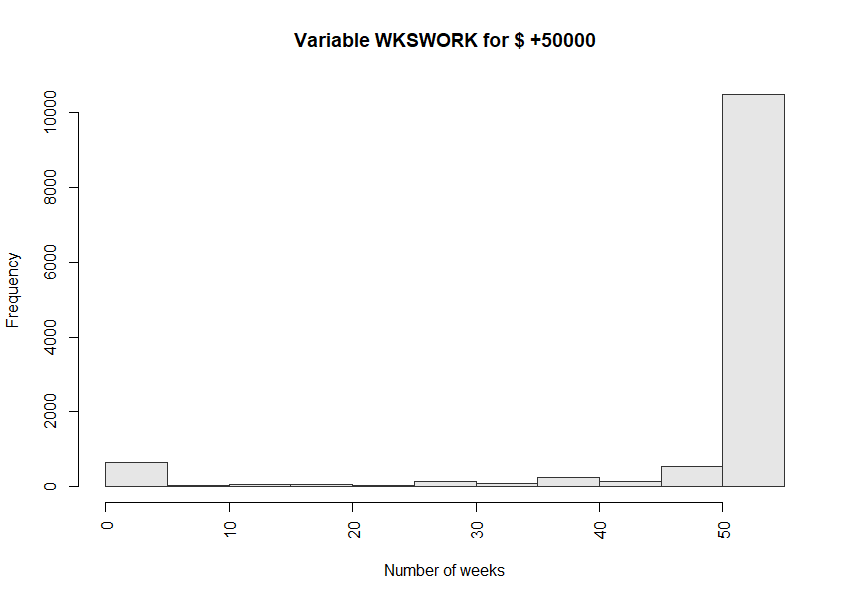
\includegraphics[width=8cm]{WKSWORKz2.png}
\end{center}
\end{enumerate} 
With the chart on the left, we can clearly see a difference of distribution between the two categories of income. If we look deeper at the second category "50000+", we notice that a large majority of these persons is working 52 weeks a year.

\newpage
\section{Conclusion}
\subsection{Challenging parts}
\noindent I spent a lot of time exploring the data set. Indeed, to be able to implement a good model, you have to know your data. I went through all the variables, check their type, the missing values and I tried to anticipate which variables will have to be pre-processed to apply one of the algorithms. Moreover, I had to make sure that R was detecting the good type for all the variables. For example, the variables "ADTIND" and "ADTOCC" are quantitative variable (they represent a code) but they have a integer as value. R was detecting these variables as "int", that is false because there is no ordinal relationship between the different codes and it could lead to a bad model.\\

\noindent Then, I had to find good alternatives to quantitative variables to implement the logistic regression algorithm. Integer encoding was not a good solution, I chose consequently one-hot encoding alternative. Nevertheless, it increased a lot the number of predictors, which means more parameters to compute. I removed arbitrarily some variables that had a high number of categories and that were summarised in a way by other variables.\\

\noindent One other challenging part was to handle the curse of dimensionality for the logistic regression model. Indeed, the algorithm didn't converge at first. To reduce the number of variables, I though about different solutions as stepwise variable selection or dimension reduction. I finally chose the lasso method, which turned out to be an efficient solution for our problem.

\noindent 
\subsection{Improvements or other ideas}
\noindent One other method that could be explored is Random Forests. I tried to implement it quickly but there was an issue with the size of our data with R. However, it could be also a good method to study deeper for the purpose of the exercise. \\

\noindent To reduce the number of variables, I could have used also the Principal Component Analysis procedure. This is a dimension reduction method. The inconvenient with this method (compared to the lasso) is that we don't used the initial variables anymore to build the model and, thus, the interpretation of the importance of the initial predictors is not possible.

\end{document}
